\documentclass{report}

\usepackage{url}
\usepackage{indentfirst}
\usepackage{float}

\usepackage{xcolor, colortbl} % Used for coloring the cells of tables
\usepackage{amsmath}
\usepackage[T1]{fontenc}
\usepackage{textcomp} % Required for upquote.
\usepackage{listings} % Used for printing source code in papers
\usepackage{microtype}

\usepackage{algorithm} % Used for writing algorithms in a paper
\usepackage[noend]{algpseudocode} % Allows psuedocode keywords (e.g., "if", "while", "for", etc.) in algorithms.

% Ensure quotes in listings are straight.
% Cleaner way to print strings in listings packages so no space symbol.
\lstset{showstringspaces=false, upquote=true} 

% eref puts parenthesis around reference, like "equation (1)"
\def\eref#1{(\ref{#1})}
% Used to generate || || (Norm) symbol for Paikin and Tal
\newcommand{\norm}[1]{\left\lVert#1\right\rVert}
\newcommand{\numbwithdegreesymbol}[1]{#1$^\circ$}

% Define the packages in the Python implementation
\newcommand{\hammoudehPuzzlePackage}{\texttt{hammoudeh\_puzzle} }
\newcommand{\paikinTalPackage}{\texttt{paikin\_tal\_solver} }

\DeclareMathOperator*{\argmax}{arg\,max} % The "*" means the limits go underneath "arg max"

% Used in the color of the table for Wrong Location
\definecolor{green}{rgb}{0,0.8,0}
\definecolor{red}{rgb}{1.0,0.0,0.0}
\definecolor{orange}{rgb}{1.0,0.6,0.2}
\definecolor{blue}{rgb}{0.0,0.0,1.0}


\usepackage{mdframed}
\usepackage[numbers,sort]{natbib}
%\usepackage[english]{babel} % Need for text wrap in table.
\usepackage{array} % Needed for centering in the table
\usepackage[export]{adjustbox} % loads also graphicx
\usepackage{graphicx}

\usepackage{hyperref} % Creates links in the PDF document.
\hypersetup{hidelinks} % Do not include boxes around links

% Defines the table of contents depth and the subsection numbering depth
\setcounter{secnumdepth}{5}
\setcounter{tocdepth}{5}

\title{   An Improved Square-Piece, Multiple
       \\ Simultaneous Jigsaw Puzzle Solver
       \\[1in]
	   CS297 Final Report}

\author{
  Zayd Hammoudeh \\
  (zayd.hammoudeh@sjsu.edu)
  }


\newcommand{\myparagraph}[1]{\paragraph{#1}\mbox{}\\}

% Skip lines after each paragraph.
\setlength\parskip{\baselineskip}

\begin{document}

\maketitle

\pagenumbering{roman}

\renewcommand{\contentsname}{Table of Contents} % Change header of TOC from "Contents" to "Table of Contents"
\tableofcontents{\protect\newpage}

\addcontentsline{toc}{section}{List of Figures}
\listoffigures
\newpage

\addcontentsline{toc}{section}{List of Tables}
\listoftables
\newpage
 
\pagenumbering{arabic}

\renewcommand\thesection{\arabic{section}}





%%%%%%%%%%%%%%%%%%%%%%%%%%%%%%%%%%%%%%%%%%%%%%%%%%%%%%%%%%%%%%%%%
%                       Introduction                            %
%%%%%%%%%%%%%%%%%%%%%%%%%%%%%%%%%%%%%%%%%%%%%%%%%%%%%%%%%%%%%%%%%

\section{Introduction}\label{sec:introduction}

Jigsaw puzzles were first introduced in the 1760s when they were made from wood; their name originated from the fact that jigsaws were used to carve the wooden pieces.   The 1930s saw the introduction of the modern jigsaw puzzle where an image was printed on a cardboard sheet that was cut into a set of interlocking pieces \cite{williams1990, williams2004}.  Although jigsaw puzzles had been solved by children for centuries, it was not until 1964 that the first automated jigsaw puzzle solver was proposed by Freeman \& Gardner \cite{freeman1964}; that solver could only solve nine piece puzzles.  While an automated jigsaw puzzle solver may seem trivial, the problem has been shown by Altman \cite{altman1990} and Demaine \& Demaine \cite{demaine2007} to be strongly NP-complete when pairwise compatibility between pieces is not a reliable metric for determining adjacency.

Jig swap puzzles are a specific type of jigsaw puzzle where all pieces are equally sized, non-overlapping squares.  Jig swap puzzles are substantially more difficult to solve since piece shape cannot be considered when determining affinity between pieces.  Rather, only the image information on each individual piece is used when solving the puzzle.  

Solving a jigsaw puzzle simplifies to reconstructing an object from a set of component pieces.  As such, techniques developed for jigsaw puzzles can be generalized to many practical problems.  Examples where jigsaw puzzle solving strategies have been used include: reassembly of archaeological artifacts \cite{brown2008, koller2006}, forensic analysis of deleted files \cite{garfinkel2010}, image editing \cite{cho2008}, reconstruction of shredded documents \cite{zhu2008}, DNA fragment reassembly \cite{marande2007}, and speech descrambling \cite{zhao2007}.  In most of these practical applications, the original, also known as ``ground-truth,'' input is unknown.  This significantly increases the difficulty of the problem as the overall structure of the complete solution must be determined solely from the bag of component pieces.

This thesis proposes an improved multiple simultaneous, jig swap puzzle solver.  What is more, it defines a set of new metrics for measuring the quality of outputs from such solvers.  Lastly, this thesis proposes enhancements to existing techniques to improve solver performance on computer generated images.



%%%%%%%%%%%%%%%%%%%%%%%%%%%%%%%%%%%%%%%%%%%%%%%%%%%%%%%%%%%%%%%%%
%                       Previous Work                           %
%%%%%%%%%%%%%%%%%%%%%%%%%%%%%%%%%%%%%%%%%%%%%%%%%%%%%%%%%%%%%%%%%

\pagebreak
\section{Previous Work}\label{sec:previousWork}

Computational jigsaw puzzle solvers have been studied since the 1960s when Freeman \& Gardner proposed a solver that relied only on piece shape and could puzzles with up to nine pieces \cite{freeman1964}.  Since then, the focus of research has gradually shifted from traditional jigsaw puzzles to jig swap puzzles.  

Cho \textit{et. al.} \citep{cho2010} proposed in 2010 one of the first modern computational jig swap puzzle solvers; their approach relied on a graphical model built around a set of one or more ``anchor piece(s)'', which are pieces whose position is fixed in the correct location before the solver began.  Cho \textit{et. al.}'s solver required that the user specify the puzzle's actual dimensions.  Future solvers would improve on Cho \textit{et. al.}'s results while simultaneously reducing the amount of information (beyond the set of pieces) passed to the solver.

A significant contribution of Cho \textit{et. al.} is that they were first to use the LAB  (\underline{L}ightness and the \underline{A}/\underline{B} opponent color dimensions) colorspace to encode image pixels (as opposed to standards such as RGB or CMYK).  LAB was selected due to its property of normalizing the lightness and color variation across all three dimensions.  Cho \textit{et. al.} also proposed a measure for quantifying the pairwise distance between two puzzle pieces that became the basis of most of the future work (see Section~\ref{sec:piecePairwiseAffinity}).  

Pomeranz \textit{et. al.} \cite{pomeranz2011} proposed an iterative, greedy jig swap puzzle solver in 2011.  Their solver did not rely on anchor pieces, and the only information passed to the solver were the pieces, their orientation, and the size of the puzzle.  Pomeranz \textit{et. al.} also generalized and improved on Cho \textit{et. al.}'s piece pairwise distance measure by proposing a ``predictive distance measure''.  Finally, Pomeranz \textit{et. al.} introduced the concept of ``best buddies'', which are any two pieces that are more similar to each other than they are to any other piece.  Best buddies have served as both an estimation metric for the quality of solver result as well as the foundation of some solvers' placers \cite{paikin2015}.

An additional key contribution of Pomeranz \textit{et. al.} is the creation of three image benchmarks.  The first benchmark is comprised of twenty 805 piece images; the size of the images in the second and third benchmarks is 2,360 and 3,300 pieces respectively.

In 2012, Gallagher \cite{gallagher2012} formally categorized jig swap puzzles into three primary types.  The following is Gallagher's proposed terminology; his nomenclature is used throughout this thesis.

\begin{itemize}

	\item \textbf{Type~1 Puzzle}: The dimension of the puzzle (i.e., the width and height of the ground-truth image in number of pixels) is known.  The orientation of each piece is also known, which means that there are exactly four pairwise relationships between any two pieces.  A single anchor piece, with a known, correct, location is required with additional anchor pieces being optional.  This type of puzzle is used by \cite{cho2010, pomeranz2011}.
	
	\item \textbf{Type~2 Puzzle}: This is an extension of a Type~1 puzzle, where pieces may be rotated in \numbwithdegreesymbol{90} increments (e.g., \numbwithdegreesymbol{0}, \numbwithdegreesymbol{90}, \numbwithdegreesymbol{180}, or \numbwithdegreesymbol{270}); in comparison to a Type~1 puzzle, this change alone increases the number of possible solutions by a factor of $4^n$, where $n$ is the number of pieces in the puzzle.  What is more, no piece locations are known in advance; this change eliminates the use of anchor piece(s).  Lastly, the dimensions of the ground-truth image may be unknown.
	
	\item \textbf{Type 3 Puzzle}: All puzzle piece locations are known and only the rotation of the puzzle pieces is unknown.  This is the least computationally complex of the three puzzle variants and is generally considered the least interesting.  Type 3 puzzles are not explored as part of this thesis.

\end{itemize}

Sholomon \textit{et. al.} \cite{sholomon2013} in 2013 proposed a genetic algorithm based solver for Type~1 puzzles.  By moving away from the greedy approach used by Pomeranz \textit{et. al.}, Sholomon \textit{et. al.}'s approach is more immune to suboptimal decisions early in the placement process. Sholomon \textit{et. al.}'s algorithm is able to solve puzzles of significantly larger size than previous techniques (e.g., greater than 23,000 pieces).  What is more, Sholomon \textit{et. al.} defined three new large image (e.g., 5,015, 10,375, and 22,834 piece) benchmarks \cite{sholomonBenchmarkImages}.

Paikin \& Tal \cite{paikin2015} published in 2015 a greedy solver that handles both Type~1 and Type~2 puzzles, even if those puzzles are missing pieces.  What is more, their algorithm is one of the first to support solving multiple jig swap puzzles simultaneously.  This entails mixing the pieces from multiple different puzzles together into a single, merged set; hence, the algorithm has no information about the source puzzle for each piece.  The solver then attempts to reconstruct the original set of distinct puzzles from the bag of pieces.

Paikin \& Tal's algorithm was used as the basis for much of this thesis and is discussed in significant depth in Section~\ref{sec:paikinTalSolver}.














%%%%%%%%%%%%%%%%%%%%%%%%%%%%%%%%%%%%%%%%%%%%%%%%%%%%%%%%%%%%%%%%%
%              Puzzle Piece Pairwise Affinity                   %
%%%%%%%%%%%%%%%%%%%%%%%%%%%%%%%%%%%%%%%%%%%%%%%%%%%%%%%%%%%%%%%%%

\pagebreak
\section{Puzzle Piece Pairwise Affinity}\label{sec:piecePairwiseAffinity}

Pairwise affinity quantifies the similarity between the sides of two puzzle pieces.  $D(x_i, s_a, x_j, s_b)$ and $C(x_i, s_a, x_j, s_b)$ represent the distance and compatibility (i.e., similarity) respectively between side $s_a$ of puzzle piece $x_i$ and side $s_b$ of puzzle piece $x_j$.  

\subsection{Cho \textit{et. al.} Pairwise Affinity}\label{sec:choPairwiseAffinity}

As mentioned in section \ref{sec:previousWork}, Cho \textit{et. al.} \cite{cho2010} proposed one of earliest edge-based pairwise affinity measures for two puzzle pieces.  Equation~\eref{eq:choPairwise} defines the distance between the right side, $R$, of piece $x_i$ and the left side, $L$, of piece $x_j$ using Cho \textit{et. al.}'s approach.  Note that $K$ is both the width and height of a puzzle piece in number of pixels.\footnote{Cho \textit{et. al.} used 7 for $K$.}

\begin{equation} \label{eq:choPairwise}
D(x_i,R,x_j,L) = \sum_{k=1}^{K}\sum_{d=1}^{3}(x_i(k,K,d) - x_j(k,1,d))^2
\end{equation}

Since the LAB colorspace has three dimensions (e.g., lightness and A/B opponent colors), $d$ ranges between $1$ and $3$.  $x_i(k,K,d)$ represents the LAB value in dimension ``$d$'' for the pixel in row ``$k$'' and column ``$K$'' in puzzle piece $x_i$.

\subsection{Pomeranz \textit{et. al.} Pairwise Affinity}\label{sec:pomeranzPairwiseAffinity}

One of the disadvantages of Cho \textit{et. al.}'s metric is that it simply squares the difference between the pieces' pixel values.  In some cases, solver performance may improve if a different exponent is used.  Pomeranz \textit{et. al.} in \cite{pomeranz2011} generalize Equation~\eref{eq:choPairwise} using the $(L_{p})^{q}$ norm as shown in Equation~\eref{eq:pomeranzPairwise}.\footnote{Pomeranz \textit{et. al.} used 28 for $K$.  This has become the standard in subsequent papers.}

\begin{equation} \label{eq:pomeranzPairwise}
D(x_i,R,x_j,L) = \bigg(\sum_{k=1}^{K}\sum_{d=1}^{3}(|x_i(k,K,d) - x_j(k,1,d)|)^p\bigg)^{\frac{q}{p}}
\end{equation}

\noindent
Equation~\eref{eq:pomeranzPairwise} is identical to that of Cho \textit{et. al.} when $p$ and $q$ are equal to $2$.

Another disadvantage of the metric proposed by Cho \textit{et. al.} is that it only considers border pixels.  Hence, if there is a gradient in the ground-truth image, two pieces may appear artificially dissimilar.  To address this issue, Pomeranz \textit{et. al.} proposed predictive compatibility; Equation~\eref{eq:pomeranzPredCompat} is the predictive compatibility between the right side, $R$, of piece $x_i$ and the left side, $L$, of piece $x_j$.  

\begin{equation} \label{eq:pomeranzPredCompat}
\begin{split}
C(x_i,R,x_j,L) = \sum_{k=1}^{K}\sum_{d=1}^{3}\Big[ ([2x_i(k, K, d) - x_i(k, K-1, d)] - x_j(k, 1, d))^p \\ - ([2x_j(k, 1, d) - x_i(k, 2, d)] - x_i(k, K, d))^p\Big]^{\frac{q}{p}}
\end{split}
\end{equation}

By including in Equation~\eref{eq:pomeranzPredCompat} the difference between the column of pixels adjacent to each edge, predictive compatibility adjusts for local gradients across puzzle pieces.

\subsection{Paikin \& Tal Pairwise Affinity}\label{sec:paikinPairwiseAffinity}

Paikin \& Tal in \cite{paikin2015} used Pomeranz \textit{et. al.}'s predictive compatibility as the foundation of their asymmetric distance measure, which is shown in Equation~\eref{eq:paikinAsymDistance}.

\begin{equation} \label{eq:paikinAsymDistance}
D(x_i,R,x_j,L) = \sum_{k=1}^{K}\sum_{d=1}^{3} \norm{[2x_i(k, K, d) - x_i(k, K-1, d)] - x_j(k, 1, d)}
\end{equation}

Paikin \& Tal set $p$ and $q$ from Equation~\eref{eq:pomeranzPairwise} equal to 1 as it both only increased the accuracy of their solver and significantly reduced the computational time.  It is important to note that since this distance is asymmetric, in most cases $D(x_i,R,x_j,L)$ does not equal $D(x_j,L,x_i,R)$.

Pomeranz \textit{et. al.} only considered the relationship between two individual pieces when determining pairwise compatibility.  In images (or areas of images) with little variation (e.g., an all white image), non-adjacent puzzle pieces may have artificially low pairwise distances.  Paikin \& Tal's asymmetric compatibility, shown in Equation~\eref{eq:paikinAsymCompatibility}, corrects for this.  $secondD(x_i,R)$ is the second best asymmetric distance between the right side of piece $x_i$ and all other pieces. 

\begin{equation} \label{eq:paikinAsymCompatibility}
C(x_i,R,x_j,L) = 1 - \frac{D(x_i,R,x_j,L)}{secondD(x_i,R)}
\end{equation}

\noindent
By normalizing compatibility with respect to the second best distance, pairings that have uniquely high compatibility are boosted, and speciously high compatibility pairings from areas of the image with low variation are penalized.

\subsubsection{Improved Asymmetric Compatibility}\label{sec:hammoudehPairwiseAffinity}

It is expected that images generated from an analog input (e.g., a photograph), will have some degree of natural variation due to: brightness, the object itself, and the capture sensor.  In contrast, such variation can be trivially removed in images generated or manipulated by computers; this includes images that are a single, solid color or object(s) shown in front of a solid background.

\begin{figure}
\centering
\fbox{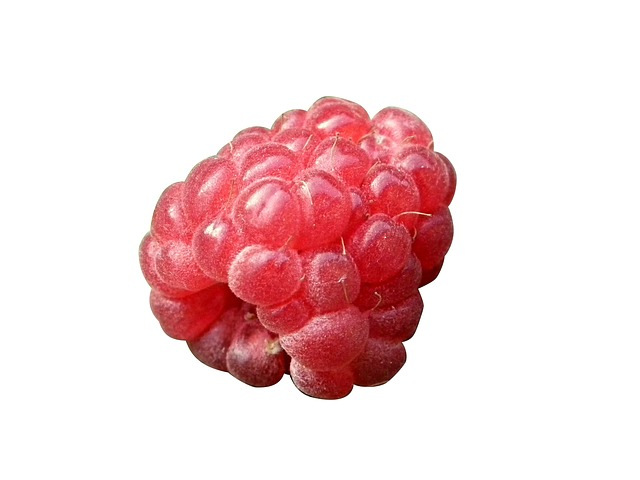
\includegraphics[width=50mm]{./images/raspberry_pixabay.jpg}}
\caption{A Computer Manipulated Image with Misleadingly High Asymmetric Compatibility due to a White Background}
\label{fig:objectWhiteBackground}
\end{figure}

Figure~\ref{fig:objectWhiteBackground} shows a berry in front of a white background; the puzzles pieces along the edge of the image and in the background have all white borders.  Hence, regardless of which of the three previously described metrics is used, the distance between all of these pieces' sides is zero.  What is more, Paikin \& Tal do not explicitly define how to handle asymmetric compatibility for such cases.  Therefore, to better handle computer generated images, this thesis proposes an enhanced definition of asymmetric compatibility shown in Equation~\eref{eq:hammoudehAsymCompatibility}.  

\begin{equation} \label{eq:hammoudehAsymCompatibility}
C(x_i,s_a,x_j,s_b)= \begin{cases} 
	1 - \frac{D(x_i,s_a,x_j,s_b)}{secondD(x_i,s_a)} & secondD(x_i,s_a) \ne 0
\\
	-\alpha & secondD(x_i,s_a) = 0
\end{cases} 
\end{equation}

\noindent
Note that $\alpha$ is a tunable, penalty factor representing low compatibility.


\subsection{Best Buddies}\label{sec:bestBuddies}

Pomeranz \textit{et. al.} defined that two pieces, $x_i$ and $x_j$ are best buddies on their respective sides $s_a$ and $s_b$ if and only if they are more compatible (i.e., similar) to each other than they are to any other piece.  This is shown formally in Equation~\eref{eq:pomeranzBestBuddyDefinition}.  The definition of best buddies is identical irrespective of the compatibility function used.

\begin{equation} \label{eq:pomeranzBestBuddyDefinition}
\centering
\begin{split}
	\begin{matrix}
		\forall{x_{k} \in \{Pieces\}}\forall{s_c}~C(x_i, s_a, x_j, s_b) \geq C(x_i, s_a, x_k, s_c)
		\\
		\\
		\textnormal{and}
		\\
		\\
		\forall{x_{k} \in \{Pieces\}}\forall{s_c}~C(x_j, s_b, x_i, s_a) \geq C(x_j, s_b, x_k, s_c)
	\end{matrix}
\end{split}
\end{equation}

\noindent
$\{Pieces\}$ represents the set of all pieces in the puzzle, and $s_c$ is one of the four sides of piece $x_k$.

It is relatively rare that two pieces are best buddies and are not actually neighbors \cite{paikin2015}.  When considering all sides of a piece, it is rarer still that a piece has more non-neighbor best buddies than neighbor best buddies.  These attributes make best buddies a critical tool for many solvers.

\subsubsection{Unique Best Buddies}\label{sec:improvedBestBuddies}

It is relatively unlikely that there will be a meaningful number pieces that have multiple best buddies on the same side if the input to the solver is a photograph.  However, similar to the phenomenon described in Section~\ref{sec:hammoudehPairwiseAffinity}, multiple best buddies may occur in computer generated or computer manipulated images.  In such cases, best buddies become a far less discerning tool for determining piece adjacency.  This thesis addresses this by modifying the definition of best buddies as shown in Equation~\eref{eq:hammoudehBestBuddyDefinition}.

\begin{equation} \label{eq:hammoudehBestBuddyDefinition}
\centering
\begin{split}
	\begin{matrix}
		\forall{x_{k \ne j} \in \{Pieces\}}\forall{s_c}~C(x_i, s_a, x_j, s_b) > C(x_i, s_a, x_k, s_c)
		\\
		\\
		\textnormal{and}
		\\
		\\
		\forall{x_{k \ne i} \in \{Pieces\}}\forall{s_c}~C(x_j, s_b, x_i, s_a) > C(x_j, s_b, x_k, s_c)
	\end{matrix}
\end{split}
\end{equation}

Rather than relying on best buddies being ``greater than or equal'' to all other pieces as in Equation~\eref{eq:pomeranzBestBuddyDefinition}, the modified requirement is that pairings must be strictly ``greater than.''  Hence, best buddy pairings are exclusive.

\subsubsection{Visualizing Best Buddies}\label{sec:visualizingBestBuddies}

There is currently no standard for visualizing an image's best buddies.  This thesis proposes such a standard for the first time.  As a nomenclature, any best buddies that are neighbors in the ground-truth image are referred to as ``adjacent best buddies'' while any best buddies that are not neighbors are referred to as ``non-adjacent best buddies.''

In a jig swap puzzle, a piece may have best buddies on up to four sides (since the pieces are square).  As such, each piece in the best buddy visualization is divided into four isosceles triangles; the base of each triangle is along the side of the puzzle piece whose best buddy is being represented.  A puzzle piece's four isosceles triangles all share a common, non-base vertex at the piece
s center.  

Figure~\ref{fig:bestBuddyVisualization} shows an image and its best buddy visualization denoted as ``(b)''. The color scheme for the different best buddy relationships is shown in Table~\ref{tab:bestBuddyColors}.


\begin{figure}
  \begin{tabular}{ >{\centering\arraybackslash}m{2.2in} >{\centering\arraybackslash}m{2.2in} }
     \fbox{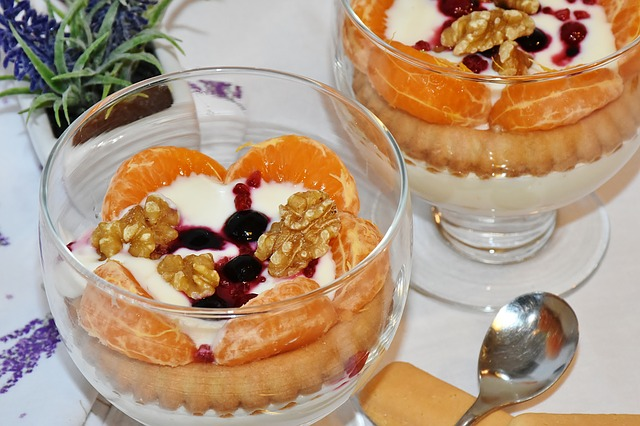
\includegraphics[width=50mm]{./images/dessert_pixabay.jpg}}  & \fbox{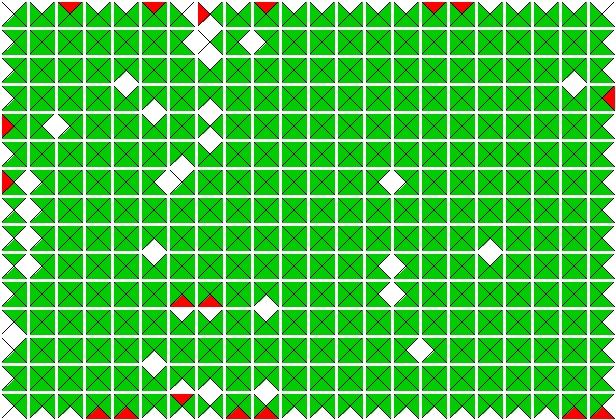
\includegraphics[width=50mm]{./images/dessert_best_buddy_visualization.jpg}}
     \\~\\
     (a) Original Image & (b) Best Buddy Visualization
  \end{tabular}
\caption{Visualization of Best Buddies in an Image}
\label{fig:bestBuddyVisualization}
\end{figure}


\begin{table}
\begin{center}
  \begin{tabular}{ | >{\centering\arraybackslash}m{0.9in} | >{\centering\arraybackslash}m{0.9in} | >{\centering\arraybackslash}m{0.9in} | >{\centering\arraybackslash}m{0.9in} | }
  
   \hline
    No Best Buddy & Non-Adjacent Best Buddy & Adjacent Best Buddy & No Piece Present  \\ \hline
	{\cellcolor{white}~} & {\cellcolor{red}~} & {\cellcolor{green}~} & {\cellcolor{black}~}  \\
	{\cellcolor{white}~} & {\cellcolor{red}~} & {\cellcolor{green}~} & {\cellcolor{black}~}  \\
 \hline

  \end{tabular}
\end{center}
\caption{Color Scheme for Puzzles Piece Sides in Best Buddy Visualizations}\label{tab:bestBuddyColors}
\end{table}

\subsubsection{Interior and Exterior Best Buddies}\label{sec:interiorExteriorBestBuddies}

In previous research, all best buddies (in particular best buddy errors) were treated the same.  However, non-adjacent best buddies are expected to naturally occur more along pieces that are on the puzzle's edge or that are next to a missing piece since those pieces lack a true neighbor; this causes those pieces to couple with unrelated pieces at a higher rate.  As an example, the image in Figure~\ref{fig:bestBuddyVisualization} has 4 interior and 14 exterior non-adjacent best buddies despite there being 16-times more interior sides. 

When using best buddy accuracy as an estimation metric, this thesis differentiates between interior and exterior best buddy errors by giving interior best buddy errors a higher weight.






%%%%%%%%%%%%%%%%%%%%%%%%%%%%%%%%%%%%%%%%%%%%%%%%%%%%%%%%%%%%%%%%%
%        Quantifying Solver Output Quality Section              %
%%%%%%%%%%%%%%%%%%%%%%%%%%%%%%%%%%%%%%%%%%%%%%%%%%%%%%%%%%%%%%%%%

\pagebreak
\section{Quantifying the Quality of a Solver Output}\label{sec:quantifyingSolverQuantify}

Cho \textit{et al.} \cite{cho2010} defined two primary metrics for quantifying the quality of a solver result namely: direct accuracy and neighbor accuracy. These metrics have been used by others including \cite{sholomon2013, pomeranz2011, paikin2015, son2014, gallagher2012}.  This section describes the existing quality metrics, their weaknesses, and proposes enhancements to these metrics to make them more meaningful for Type~2 puzzles as well as when solving multiple puzzles simultaneously.

In the final subsection, the tools developed to visualize the solver output quality are discussed.

\subsection{Direct Accuracy}\label{sec:directAccuracy}

Direct accuracy is the most na\"{\i}ve accuracy measure.  It is defined as the fraction of pieces placed in the same location in the ground-truth (i.e., original) and solved image with respect to the total number of pieces.  Equation~\eref{eq:directAccuracy} shows the formal definition of direct accuracy ($DA$), where $n$ is the total number of pieces and $c$ is the number of pieces placed in the original (i.e., correct) location.

\begin{equation} \label{eq:directAccuracy}
DA = \frac{c}{n}
\end{equation}

Direct accuracy is vulnerable to shifts in the solved image where even a few misplaced pieces can cause a significant decrease in accuracy.  This can be particularly true when the ground-truth image's dimensions are not known by the solver as shown in Section~\ref{sec:shiftableEnhancedDirectAccuracy}.

This thesis proposes two new direct accuracy metrics namely: ``Enhanced Direct Accuracy Score'' (EDAS) and ``Shiftable Enhanced Direct Accuracy Score'' (SEDAS).  They are described in the following two subsections; the complementary relationship between EDAS and SEDAS is described in the third subsection.

\subsubsection{Enhanced Direct Accuracy Score}\label{sec:enhancedDirectAccuracyScore}

The standard direct accuracy metric does not account for the possibility that there may be pieces from multiple puzzles in the same solver output.  For a given a puzzle $P_i$ in the set of input puzzles $P$ (where $P_i \in P$) and a set of solved puzzles $S$ where $S_j$ is in $S$, Enhanced Direct Accuracy Score (EDAS) is defined as shown in Equation~\eref{eq:enhancedDirectAccuracyScore}.

\begin{equation} \label{eq:enhancedDirectAccuracyScore}
EDAS_{P_i} = \argmax_{S_j \in S}\frac{c_{i,j}}{n_i + \sum_{k \ne i}(m_{k,j})}
\end{equation}

\noindent
$c_{ij}$ is the number of pieces from input puzzle $P_i$ correctly placed (with no rotation for Type~2 puzzles) in solved puzzle $S_j$ while $n_i$ is the number of pieces in puzzle $P_i$. $m_{k,j}$ is the number of pieces from an input puzzle $P_k$ (where $k \ne i$) that are also in $S_j$.

When solving only a single puzzle, EDAS and standard direct accuracy in Equation~\eref{eq:directAccuracy} are equivalent.  When solving multiple puzzles simultaneously, EDAS necessarily marks as incorrect any pieces from $P_i$ that are not in $S_j$ by dividing by $n_i$.  What is more, the summation of $m_{k,j}$ in EDAS is used to penalize for any puzzles pieces not from $P_i$.  Combined, these two factors enable EDAS to account for both extra and misplaced pieces.

It is important to note that EDAS is a score and not a measure of accuracy. While its value is bounded between 0 and 1 (inclusive), it is not specifically defined as the number of correct placements divided by the total number of placements since the denominator of Equation~\eref{eq:enhancedDirectAccuracyScore} is greater than or equal to the number of pieces in the puzzles $P_i$ and $S_j$.

\subsubsection{Shiftable Enhanced Direct Accuracy Score}\label{sec:shiftableEnhancedDirectAccuracy}

As mentioned previously, the direct accuracy decreases if there are shifts in the solved image.  In many cases, direct accuracy is overly punitive when penalizing for shifts. 

Figure~\ref{fig:directAccuracyOnePieceEffect} shows the ground-truth image and an actual solver output when the puzzle boundaries were not fixed.  Note that only a single piece is misplaced; this shifted pieces to the right one location causing the direct accuracy to drop to zero.  Had this same piece been misplaced at either the right or bottom side of the image, the direct accuracy would have been largely unaffected.  The fact that direct accuracy can give such vastly differing results for essentially the same error shows that direct accuracy can be seriously flawed.  This thesis proposes Shiftable Enhanced Direct Accuracy Score (SEDAS) to address the often misleadingly punitive nature of direct accuracy. 

\begin{figure}
  \begin{tabular}{ >{\centering\arraybackslash}m{2.2in} >{\centering\arraybackslash}m{2.2in} }
	\fbox{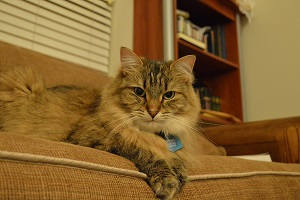
\includegraphics[width=48mm]{./images/muffins_300x200.jpg}} & \fbox{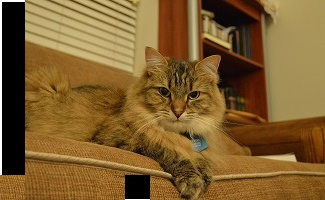
\includegraphics[width=50.1mm]{./images/muffins_300x200_type1}}
	\\ ~\\
	(a) Ground-Truth Image & (b) Solver Output
	\\ ~\\
  \end{tabular}
\caption{Solver Output where a Single Misplaced Piece Catastrophically Affects the Direct Accuracy}
\label{fig:directAccuracyOnePieceEffect}
\end{figure}

Let $d_{min}$ be the Manhattan distance between the upper left corner of the solved image and the nearest placed puzzle piece.  Also let $L$ as the set of all puzzle piece locations within distance $d_{min}$ of the upper left corner of the image.  Given that $l$ is a location in $L$ that is used as the reference point for determining the absolute location of all piece, then SEDAS is defined as shown in Equation~\eref{eq:shiftableEnhancedDirectAccuracyScore}.  

\begin{equation} \label{eq:shiftableEnhancedDirectAccuracyScore}
SEDAS_{P_i} = \argmax_{l \in L} \bigg( \argmax_{S_j \in S}\frac{c_{i,j,l}}{n_i + \sum_{k \ne i}(m_{k,j})} \bigg)
\end{equation}

\noindent
In standard definition of direct accuracy, $l$ would be the upper left corner of the image; SEDAS shifts this reference point within a radius of the upper left corner of the image in order to find a more meaningful value for direct accuracy. 

Rather than defining SEDAS based off the distance $d_{min}$, an alternative approach is to use the point in the image that maximizes Equation~\eref{eq:shiftableEnhancedDirectAccuracyScore}.  However, that approach can be significantly more computationally complex in particular on large puzzles of several thousand pieces.  Hence, this thesis' approach balances finding a meaningful direct accuracy score with computational efficiency.

\subsubsection{The Necessity to Use Both EDAS and SEDAS}\label{sec:importanceEdasSedas}

While EDAS can be misleadingly punitive, it cannot be wholly replaced by SEDAS.  Rather, EDAS and SEDAS serve complementary roles.  First, EDAS must necessarily be calculated as part of SEDAS since the upper left corner location is inherently a member of the set $L$.  Hence, there is no additional time required to calculate EDAS.  What is more, by continuing to use EDAS along with SEDAS, some shifts in the solved image may be quantified; this would not be possible if SEDAS was used alone.

\subsection{Neighbor Accuracy}\label{sec:neighborAccuracy}

Cho \textit{et al.} \cite{cho2010} defined neighbor accuracy as the ratio of the number of puzzle piece sides adjacent to the same piece's side in both the ground-truth and solved image versus the total number of puzzle piece sides.  Formally, let $q$ be the number of sides each piece has (i.e., four in a jig swap puzzle) and $n$ be the number of pieces.  If $a$ is the number of puzzle piece sides adjacent in both the ground-truth and solved images, then the neighbor accuracy, $NA$, is defined as shown in Equation~\eref{eq:neighborAccuracy}.

\begin{equation} \label{eq:neighborAccuracy}
NA = \frac{a}{n~q}
\end{equation}

Unlike direct accuracy, neighbor accuracy is largely unaffected by shifts in the solved image since it considers only a piece's neighbors and not its absolute location.  However, the standard definition of neighbor accuracy cannot encompass the case where pieces from multiple input puzzles may be present in the same solver output.  

\subsubsection{Enhanced Neighbor Accuracy Score}\label{sec:enhancedNeighborAccuracyScore}

Enhanced Neighbor Accuracy Score (ENAS) improves the neighbor accuracy metric by providing a framework to quantify the quality of a solver output when solving multiple puzzles simultaneously. 

Let $n_i$ be the number of puzzles pieces in the input puzzle $P_i$ and $a_{i,j}$ be the number of puzzle piece sides adjacent in $P_i$ and $S_j$.  If $m_{k,j}$ is the number of puzzle pieces from an input puzzle $P_k$ (where $k \ne i$) in $S_j$, then the ENAS for $P_i$ is defined as shown in Equation~\eref{eq:enhancedNeighborAccuracyScore}.

\begin{equation} \label{eq:enhancedNeighborAccuracyScore}
ENAS_{P_i} = \argmax_{S_j \in S}\frac{a_{i,j}}{q ~ (n_i + \sum_{k \ne i}(m_{k,j})}
\end{equation}

In the same fashion as the technique described for EDAS in Section~\ref{sec:enhancedDirectAccuracyScore}, ENAS divides by the number of pieces $n_i$ in input puzzle $P_i$.  By doing so, it effectively marks as incorrect any pieces from $P_i$ that are not in $S_j$.  What is more, by including a summation of all $m_{k,j}$ in the denominator of \eref{eq:enhancedNeighborAccuracyScore}, ENAS marks as incorrect any pieces not from $P_i$ that are in $S_j$.  The combination of these two factors allows ENAS to account for extra and misplaced pieces.

\subsection{Visualizing Solver Output Quality}\label{sec:visualizingSolverAccuracy}

In images with thousands of pieces, it is often difficult to visually determine the location of individual pieces that are incorrectly placed.  What is more, visual tools help developers quickly detect and fix latent bugs.

The following two subsections show the tools developed as part of this thesis for visualizing direct accuracy and neighbor accuracy.

\subsubsection{Visualizing EDAS and SEDAS}\label{sec:visualizingEdasSedas}

In standard direct accuracy, EDAS, and SEDAS, each puzzle piece is assigned a single value (i.e., correct or incorrect).  Due to that, the direct accuracy visualization represents each puzzle by a square filled with a solid color.  One additional refinement used in this thesis is to subdivide the ``incorrect'' placements into a set of subcategories organized by decreasing severity: wrong puzzle, wrong location, and wrong rotation.  Table~\ref{tab:directAccuracyColors} shows the colors assigned to puzzle pieces depending on their direct accuracy classification.

\begin{table}[h]
	\begin{center}
  		\begin{tabular}{ | >{\centering\arraybackslash}m{0.6in} | >{\centering\arraybackslash}m{0.6in} | >{\centering\arraybackslash}m{0.6in} | >{\centering\arraybackslash}m{0.6in} | >{\centering\arraybackslash}m{0.6in} | }
 \hline
    		Wrong Puzzle & Wrong Location & Wrong Rotation & Correct Location  & No Piece Present  \\ \hline
			{\cellcolor{blue}~} & {\cellcolor{red}~}  & {\cellcolor{orange}~}  & {\cellcolor{green}~} & {\cellcolor{black}~}  \\
			{\cellcolor{blue}~} & {\cellcolor{red}~}  & {\cellcolor{orange}~}  & {\cellcolor{green}~} & {\cellcolor{black}~} \\
 \hline
		\end{tabular}
	\end{center}
\caption{Color Scheme for Puzzles Pieces in Direct Accuracy Visualizations}\label{tab:directAccuracyColors}
\end{table}

Figure~\ref{fig:directAccuracyVisualization} shows a Type~2 solver output along with the associated EDAS and SEDAS visualizations. Since four puzzle pieces were erroneously placed on the left of the image, almost all pieces had the wrong location according to EDAS; the only exception is a single piece that had the right location, but wrong rotation.  In contrast, almost all pieces had the correct location in the SEDAS representation; note that the piece that had the correct location but wrong rotation in EDAS has the wrong location in SEDAS.

\begin{figure}
\centering

  \begin{tabular}{ >{\centering\arraybackslash}m{2.2in} >{\centering\arraybackslash}m{2.2in} }
  
	\fbox{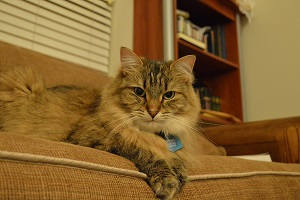
\includegraphics[width=48mm]{./images/muffins_300x200.jpg}} & \fbox{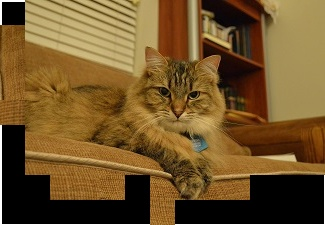
\includegraphics[width=52.1mm]{./images/muffins_300x200_type2}} \\~\\
	(a) Ground-Truth Image & (b) Type~2 Solver Output
\\~\\
	\fbox{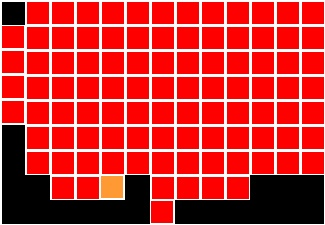
\includegraphics[width=52.1mm]{./images/muffins_300x200_type_EDAS.jpg}} & \fbox{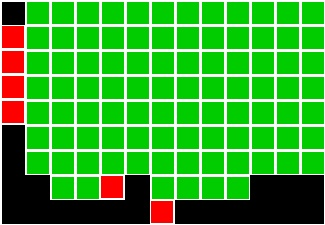
\includegraphics[width=52.1mm]{./images/muffins_300x200_type_SEDAS.jpg}}
\\~\\
	(c) EDAS Visualization & (d) SEDAS Visualization  
  \end{tabular}

\caption{Example Solver Output Visualizations for EDAS and SEDAS}
\label{fig:directAccuracyVisualization}
\end{figure}

\subsubsection{Visualizing Neighbor Accuracy}\label{sec:visualizingNeighborAccuracy}

The visualization for neighbor accuracy is very similar to the techniques described in Section~\ref{sec:visualizingBestBuddies} for visualizing best buddies where each puzzle piece is divided into four equal-sized isosceles triangles (i.e., one for each side).  The triangles are assigned colors depending on whether their neighbor in the solver output and ground-truth image match.  The visualization includes a subcategory known as ``wrong puzzle'' which is a special case that occurs when solving multiple puzzles simultaneously and some of the pieces in the solved puzzle are not from the puzzle of interest, $P_i$.  Table~\ref{tab:neighborAccuracyColors} defines the colors used to represent the different classification of puzzle piece sides in neighbor accuracy visualization.

\begin{table}[h]
\begin{center}
  \begin{tabular}{ | >{\centering\arraybackslash}m{0.6in} | >{\centering\arraybackslash}m{0.6in} | >{\centering\arraybackslash}m{0.6in} | >{\centering\arraybackslash}m{0.6in} | >{\centering\arraybackslash}m{0.6in} | }
 \hline
    Wrong Puzzle & Wrong Neighbor & Correct Neighbor  & No Piece Present  \\ \hline
	{\cellcolor{blue}~} & {\cellcolor{red}~} & {\cellcolor{green}~} & {\cellcolor{black}~}  \\
	{\cellcolor{blue}~} & {\cellcolor{red}~} & {\cellcolor{green}~} & {\cellcolor{black}~}  \\
 \hline
  \end{tabular}
\end{center}
\caption{Color Scheme for Puzzles Piece Sides in Neighbor Accuracy Visualizations}\label{tab:neighborAccuracyColors}
\end{table}

Figure~\ref{fig:neigborAccuracyVisualization} shows an actual output when solving two images simultaneously.  Note that that the puzzle of interest is the glass and stone building while the other puzzle is a rainforest house.

\begin{figure}
\centering

  \begin{tabular}{ >{\centering\arraybackslash}m{2.2in} >{\centering\arraybackslash}m{2.2in} }
  
	\fbox{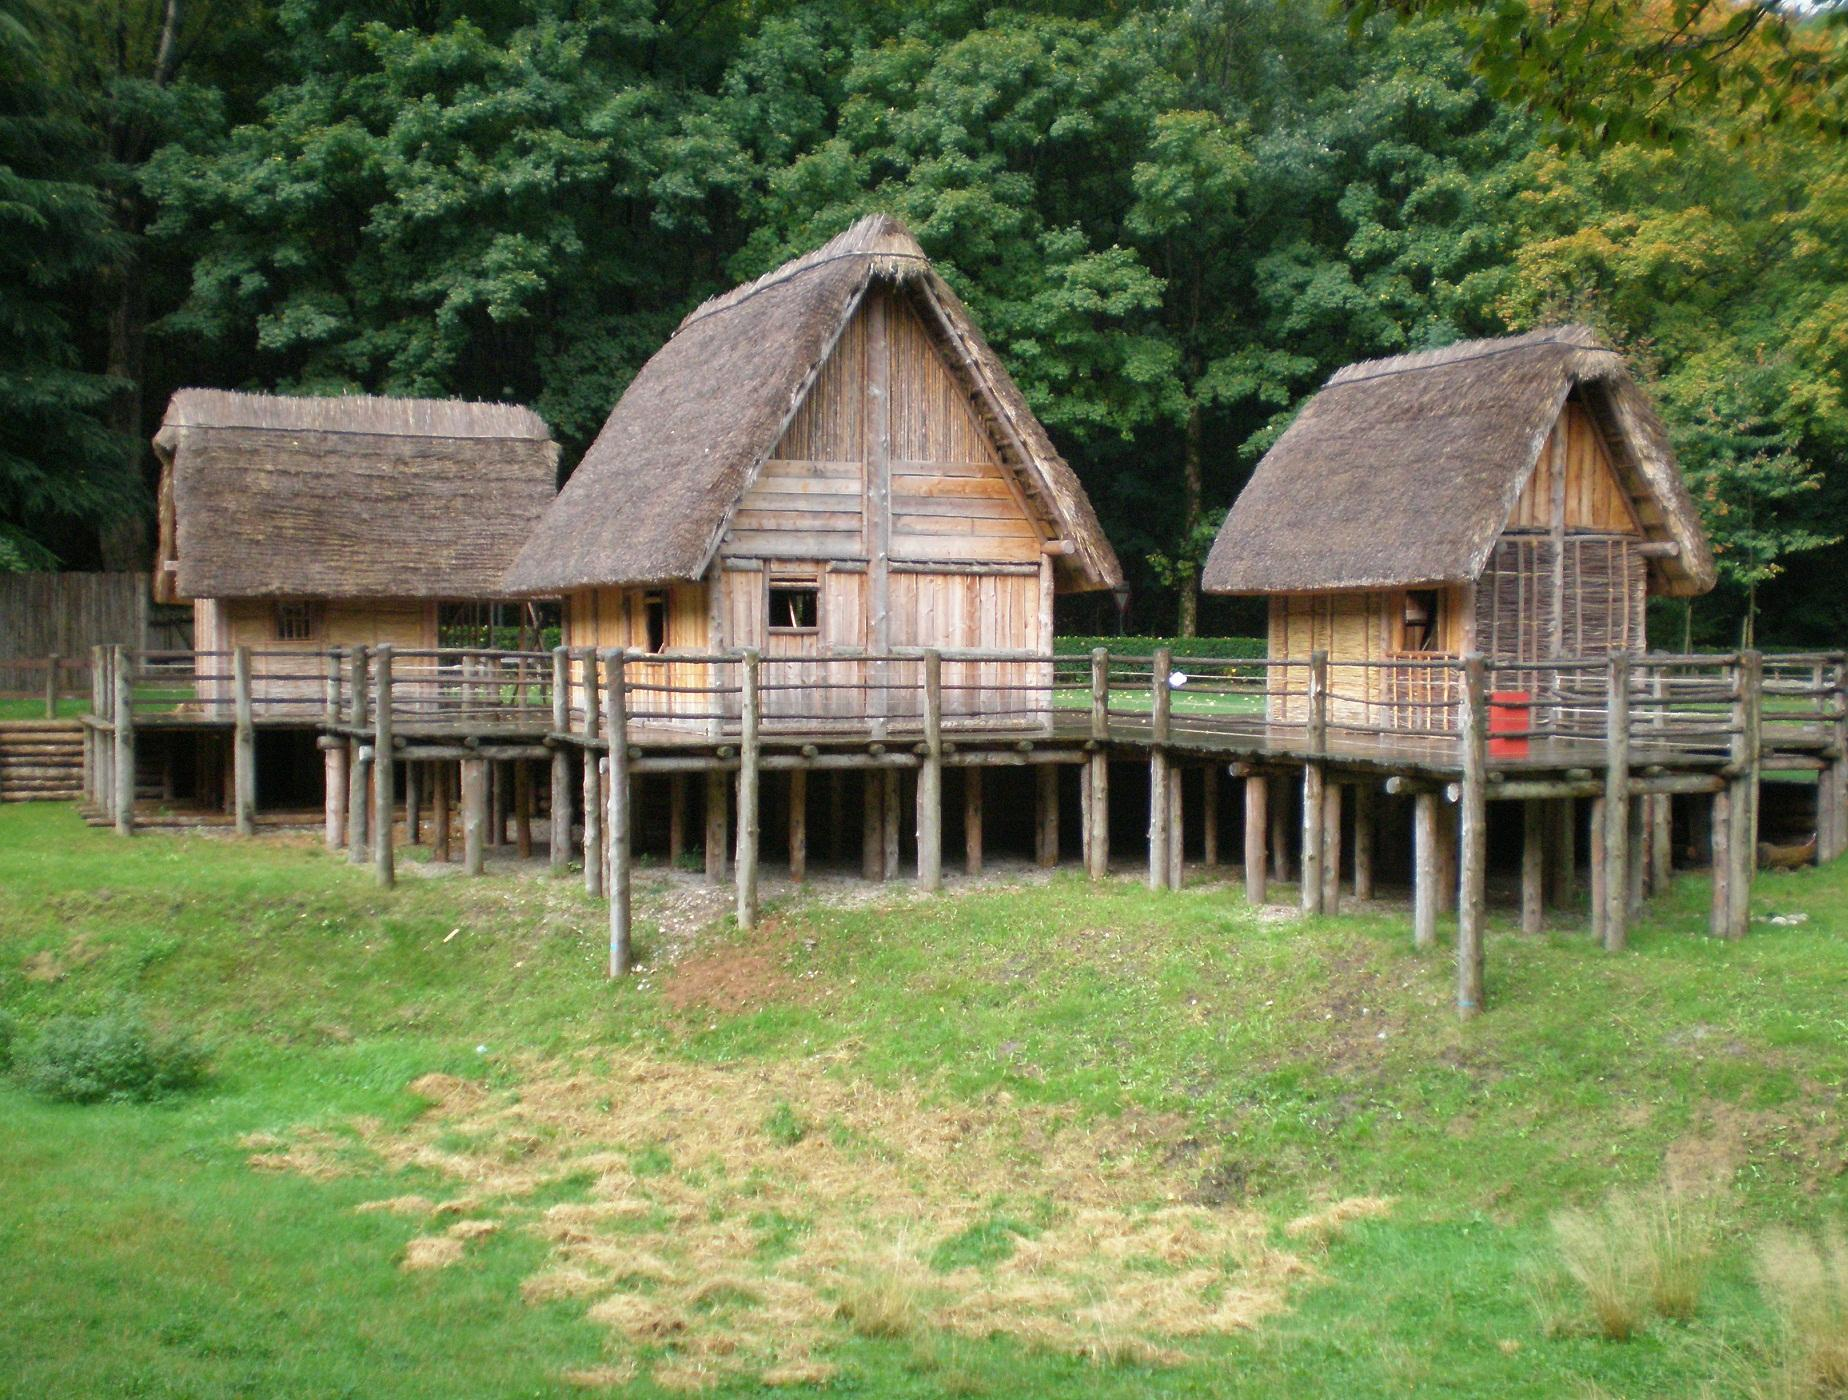
\includegraphics[width=1.7in]{./images/pomeranz_3300_1.jpg}} & \fbox{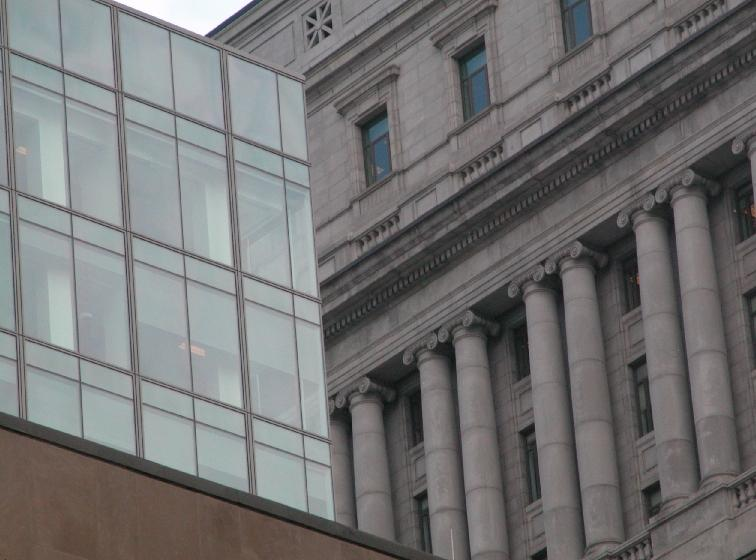
\includegraphics[width=1.5in]{./images/mcgill_20.jpg}} \\~\\
	(a) Input Image \# 1 - Rainforest House \cite{pomeranzBenchmarkImages} & (b) Input Image \# 2 - Building Exterior \cite{mcgillImageDatabase}
\\~\\
	\fbox{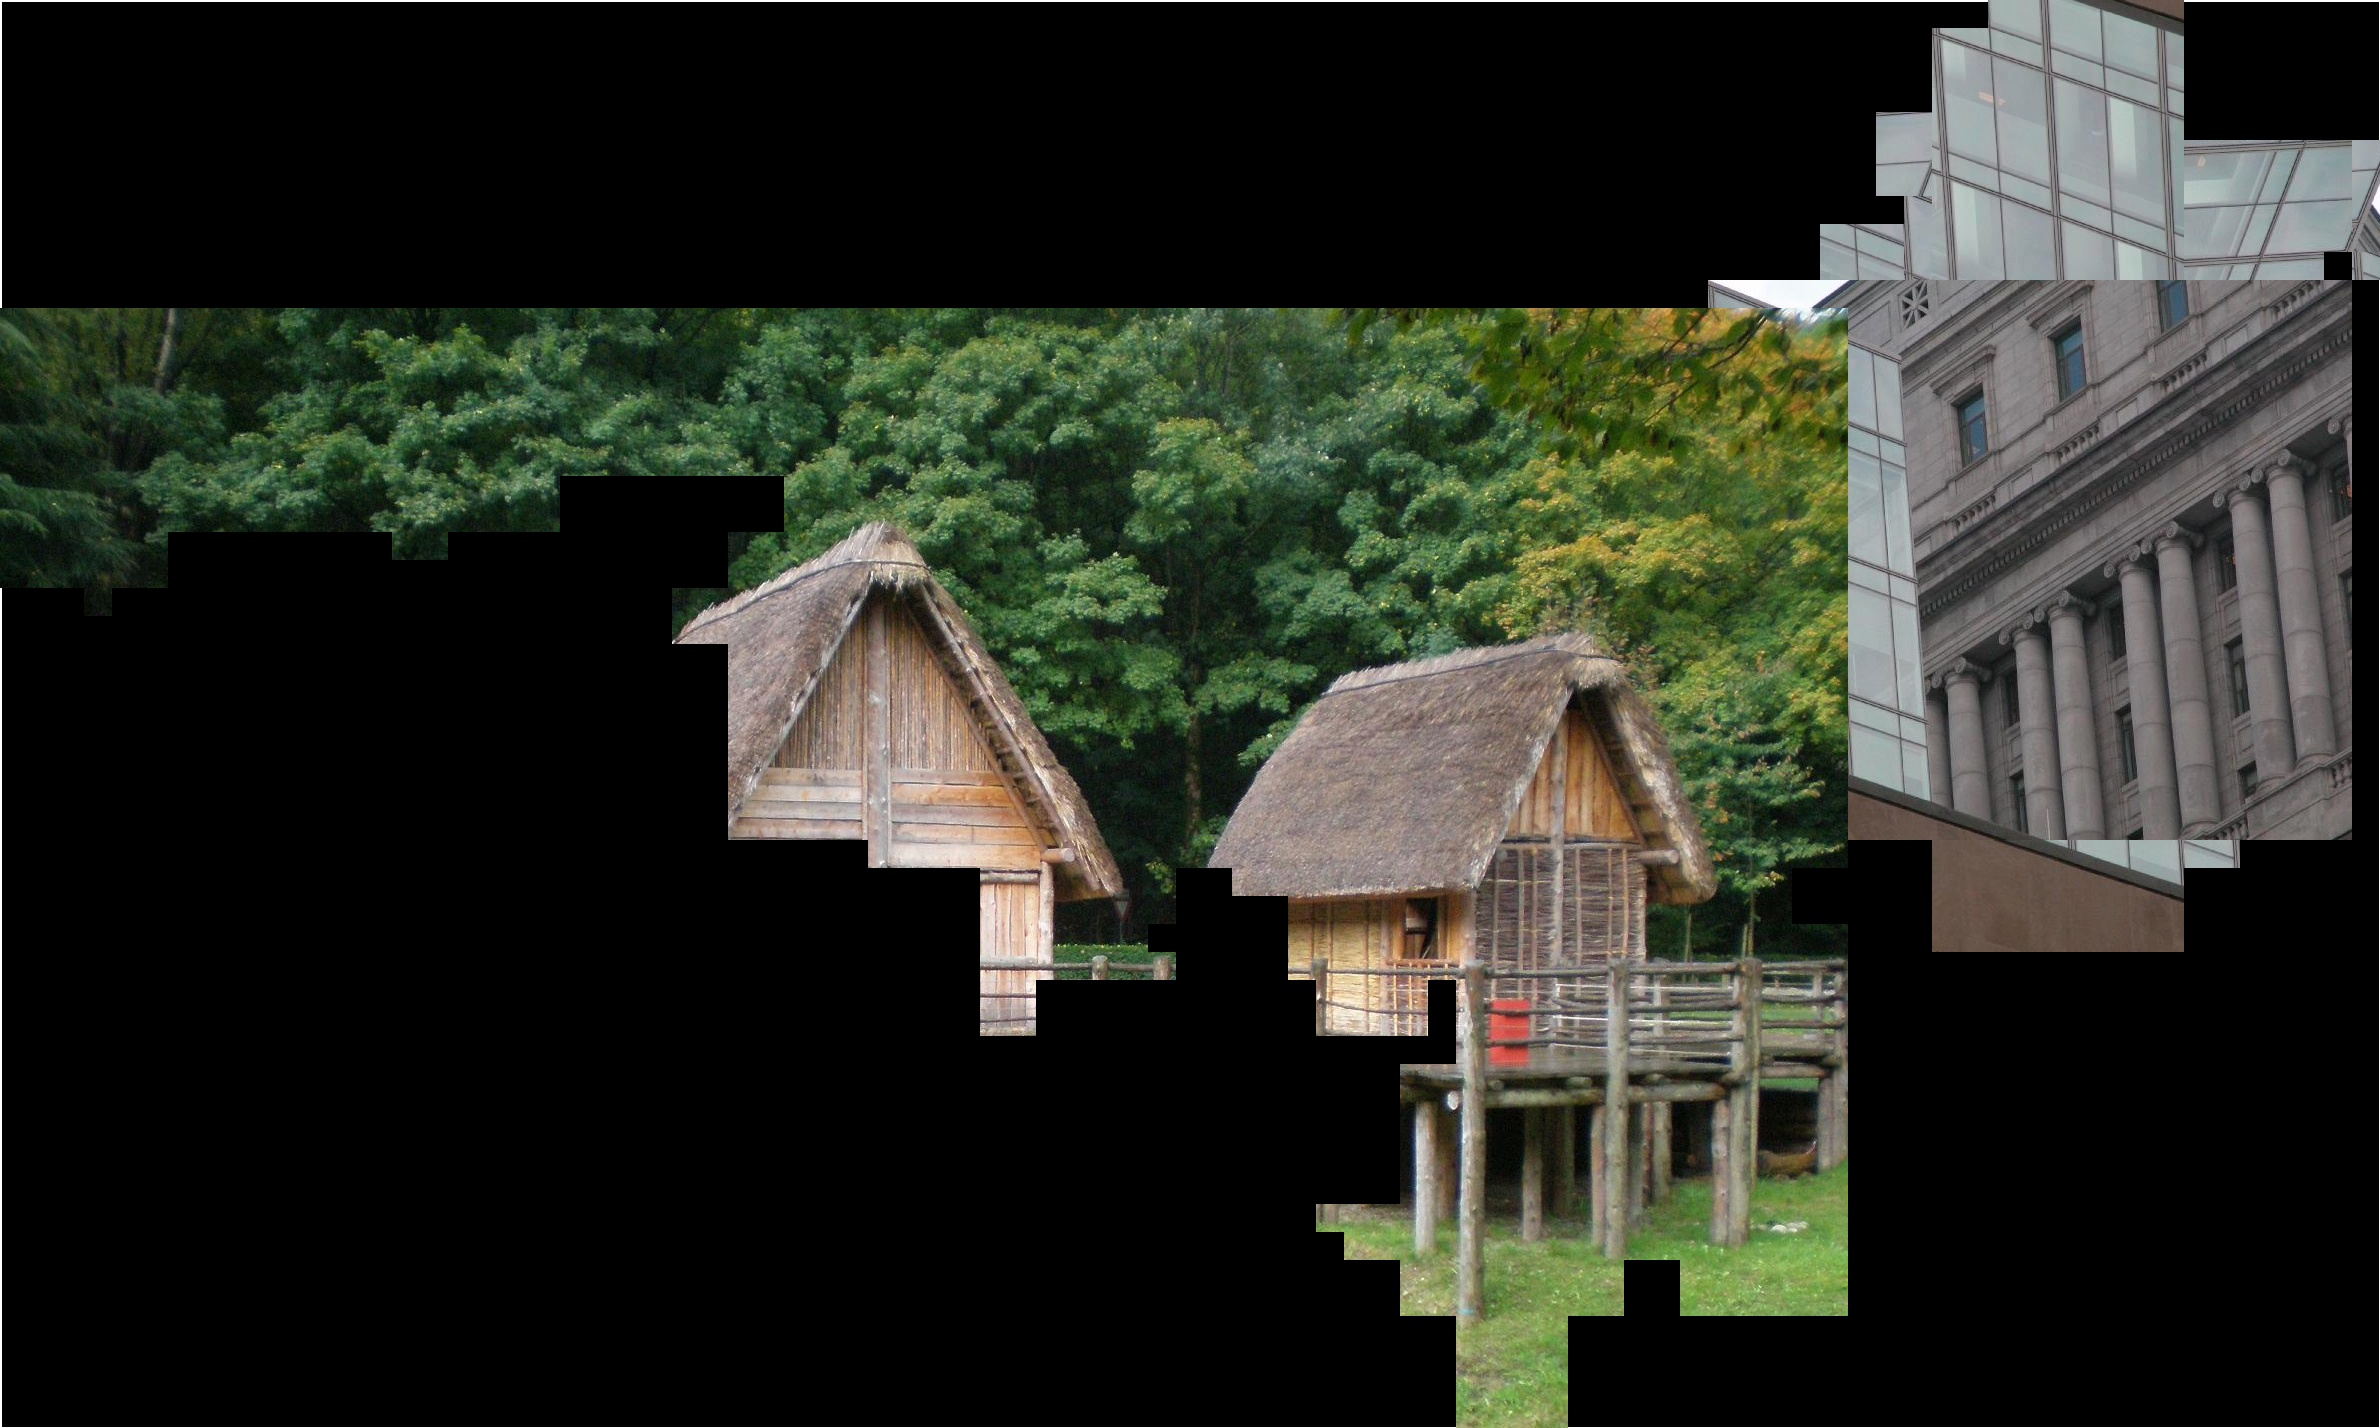
\includegraphics[width=2.1in]{./images/3300_1_mcgill_20_type_2.jpg}}
	& \fbox{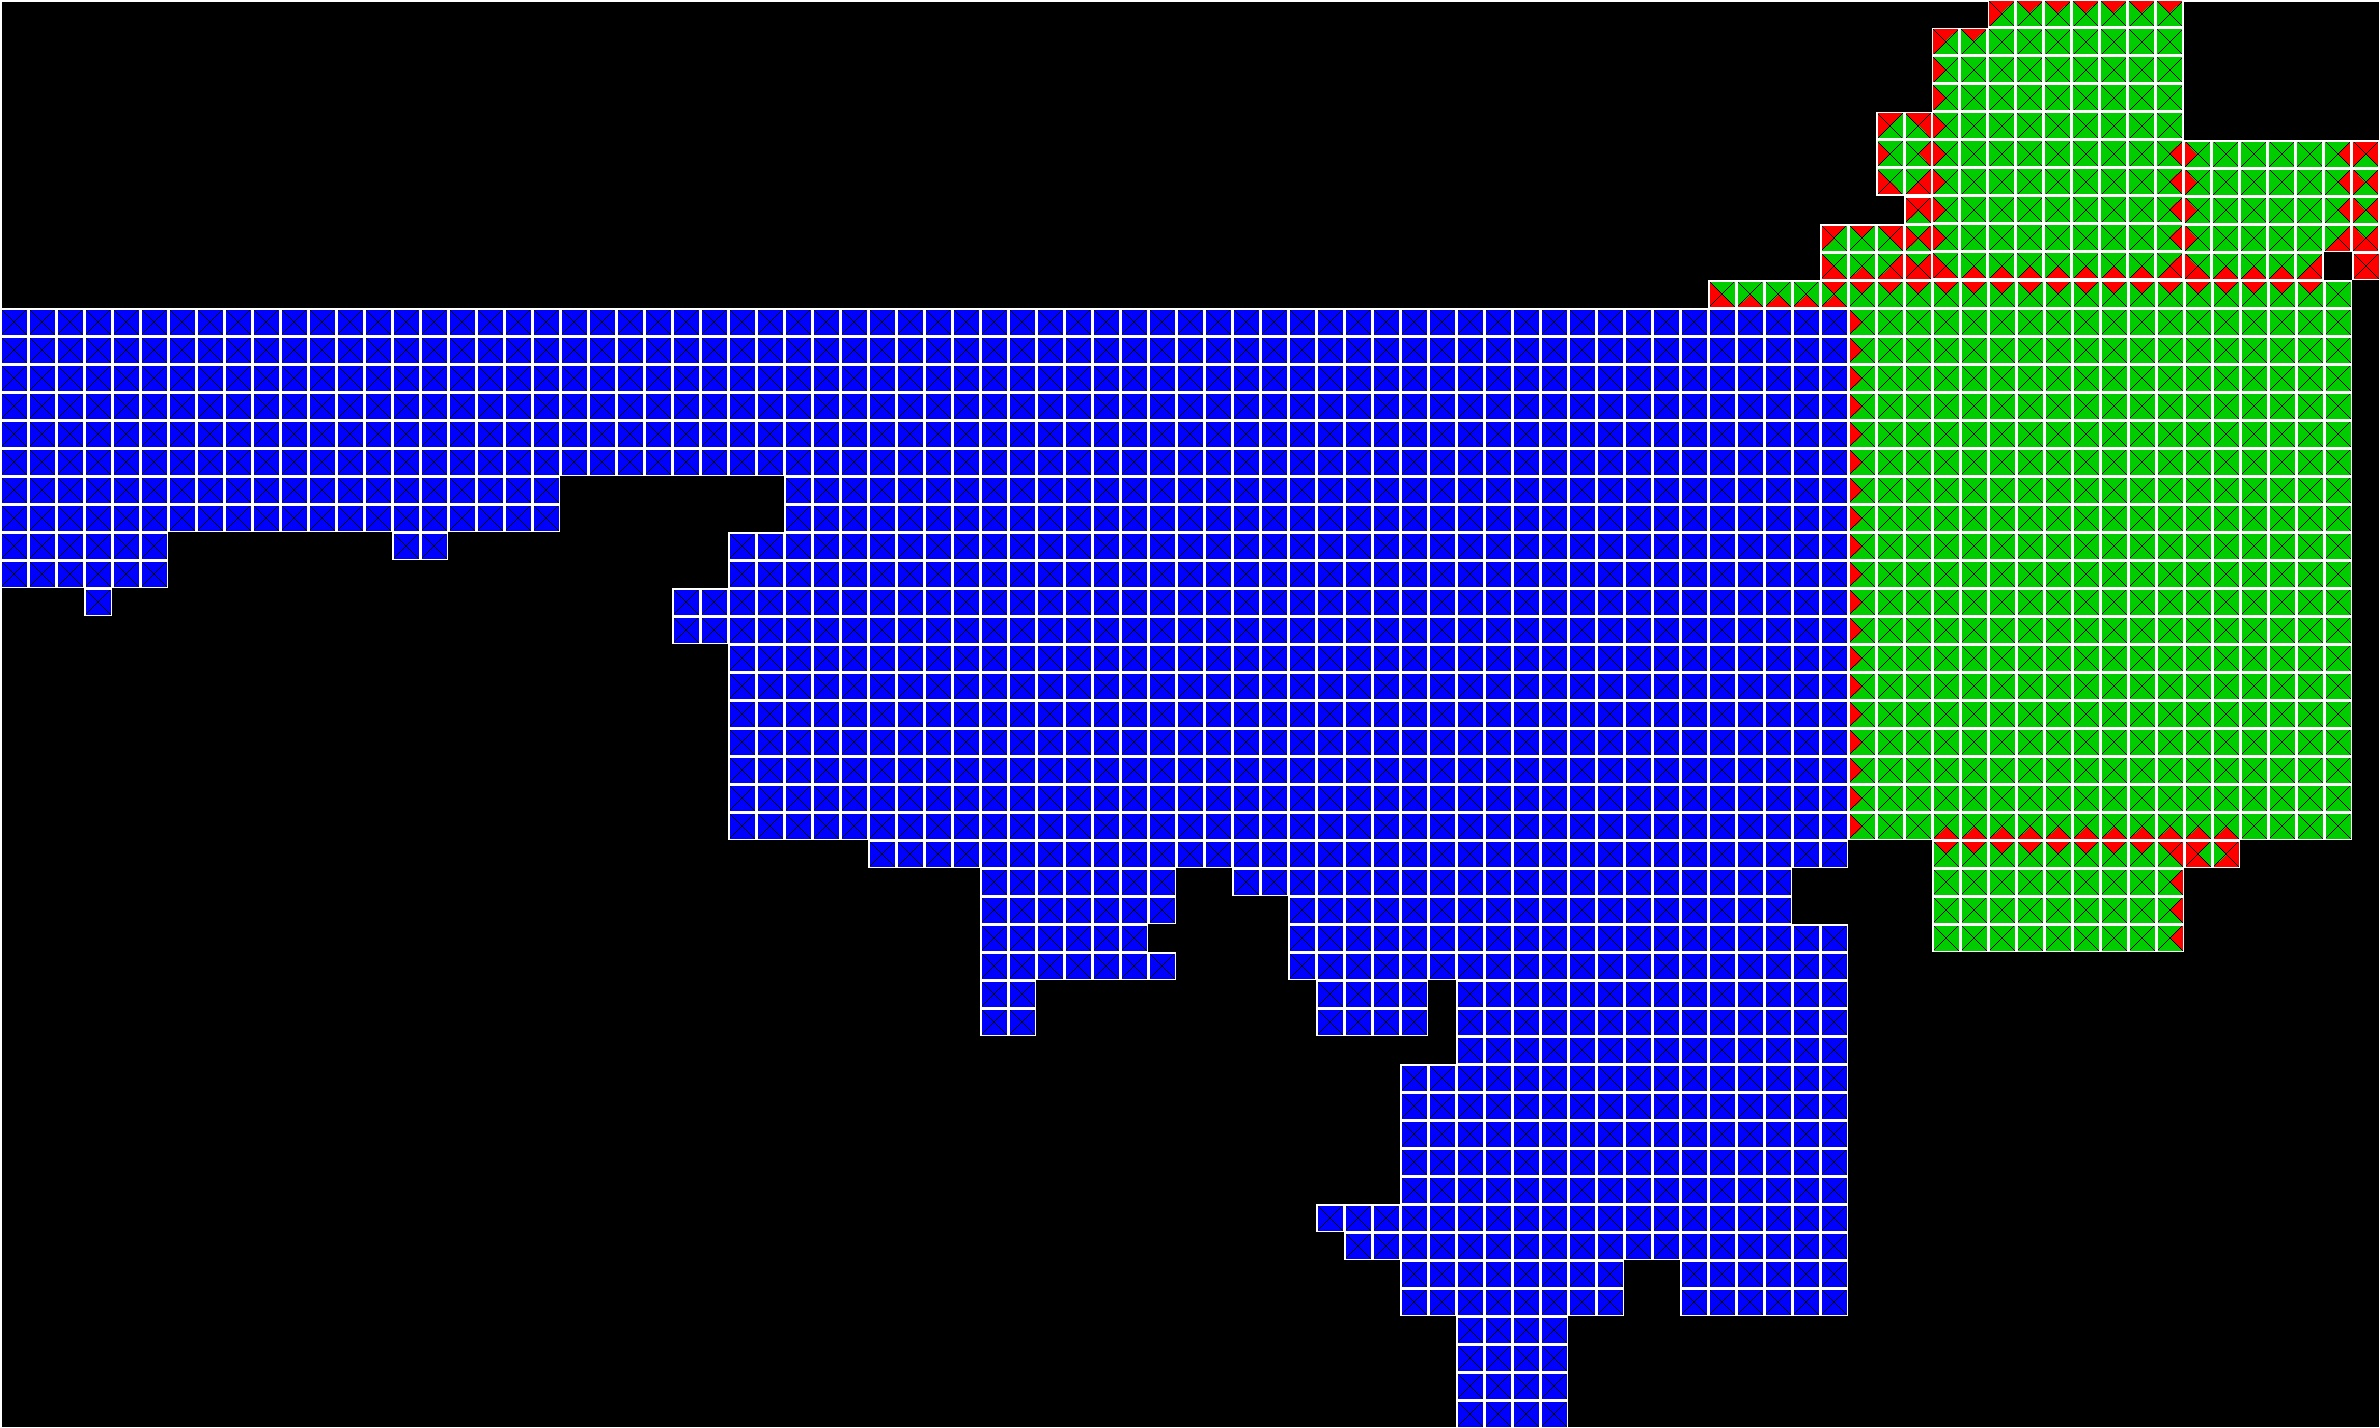
\includegraphics[width=2.1in]{./images/3300_1_mcgill_20_ENAS.jpg}}
\\~\\
	(c) Solver Output & (d) ENAS Visualization  
  \end{tabular}

\caption{Example Solver Output Visualization for ENAS}
\label{fig:neigborAccuracyVisualization}
\end{figure}

All pieces that came from the rainforest house image are shown as blue despite being assembled correctly; this is because they are not from the puzzle of interest.  All neighbors from the puzzle of interest (i.e., the glass and stone building) that are placed next to their original neighbor are represented by green triangles while all incorrect neighbors, such as those bordering the rainforest house image, are shown with red triangles.








%%%%%%%%%%%%%%%%%%%%%%%%%%%%%%%%%%%%%%%%%%%%%%%%%%%%%%%%%%%%%%%%%
%                    Paikin & Tal Solver                        %
%%%%%%%%%%%%%%%%%%%%%%%%%%%%%%%%%%%%%%%%%%%%%%%%%%%%%%%%%%%%%%%%%

\pagebreak
\section{Paikin \& Tal Solver}\label{sec:paikinTalSolver}

This section reviews the solver proposed by Paikin \& Tal \cite{paikin2015}; their Java implementation is not open-source.  As such, this section also describes a complete implementation of their approach that was developed as part of this thesis.

\subsection{Overview of Paikin \& Tal's Algorithm}\label{sec:paikinTalAlgorithm}

Paikin \& Tal's solver was inspired by the work of Pomeranz \textit{et. al.} in \cite{pomeranz2011}.  Paikin \& Tal's uses a deterministic, greedy algorithm that places the puzzle piece that has the maximum confidence score at each iteration. Paikin \& Tal's approach is able to handle puzzles of unknown size with missing pieces and where piece orientation is not known.  The only required input to the algorithm is the expected number puzzles.

Paikin \& Tal's algorithm has three distinct phases namely: inter-puzzle piece distance calculation, selection of the seed piece, and placement.  These stages are described in the following subsections.  The modification required during placement to solve multiple puzzles simultaneously is described in an additional subsection.

\subsubsection{Inter-Puzzle Piece Distance Calculation}\label{sec:paikinTalInterPieceDistance}

The first stage of Paikin \& Tal's algorithm is to calculate the inter-piece distance between all pieces.  This is done using the asymmetric distance measure described in Section~\ref{sec:paikinPairwiseAffinity}.  The distance information is stored in an $n$ by $n$ matrix (where $n$ is the number of puzzle pieces); after being initially calculated, the asymmetric distances never need to be recalculated.

As explained in Section~\ref{sec:paikinPairwiseAffinity}, Paikin \& Tal normalize the asymmetric distances using the asymmetric compatibility function in Equation~\eref{eq:paikinAsymCompatibility}.  This has the effect of amplifying truly unique pairings while penalizing speciously similar pairings that arise from low variation areas of the image.  The asymmetric compatibility is then used to find the best buddies for each piece (if any).  

The last step is to calculate the mutual compatibility ($\tilde{C}$) between pairs of pieces (e.g., $x_i$ and $x_j$), which is defined in Equation~\eref{eq:mutualCompatibility}.  $C(x_i,s_a,x_j,s_b)$ is the asymmetric compatibility between side $s_a$ of piece $x_i$ and side $s_b$ of piece $x_j$; $C(x_j,s_b,x_i,s_a)$ is defined similarly.  It is important to note that mutual compatibility is symmetric.

\begin{equation} \label{eq:mutualCompatibility}
\tilde{C}(x_i,s_a,x_j,s_b)=\tilde{C}(x_j,s_b,x_i,s_a)=\frac{C(x_i,s_a,x_j,s_b) + C(x_j,s_b,x_i,s_a) }{2}
\end{equation}

\subsubsection{Selecting the Seed Piece}\label{sec:paikinTalSeedPiece}

Similar to Pomeranz \textit{et al.}, Paikin \& Tal used a kernel growing algorithm.  Hence, a seed piece is selected, and all pieces are placed around that seed.    Since the algorithm is greedy, the selection of a poor seed can have a significant, deleterious impact on the final solution.  Due to this, Paikin \& Tal select a piece that is itself ``distinctive'' and comes from a ``distinctive region.''  

Paikin \& Tal define a seed piece as ``distinctive'' if it has best buddies on each of its sides.  To ensure that a piece comes from a distinctive region, all of the seed piece's best buddies must also have four best buddies. In a puzzle, there may be multiple pieces that satisfy the ``distinctive'' piece in a ``distinctive region'' criteria; in such cases, ties are broken by selecting the piece that has the maximum sum of mutual compatibilities with its direct neighbors.

\subsubsection{Placement}\label{sec:paikinTalPlacer}

Paikin \& Tal utilized an iterative, greedy placer that places pieces around an expanding seed.  Pseudocode for their placer is shown in Algorithm~\ref{alg:paikinTalPlacer}.  Placement continues all pieces have been placed.

\begin{algorithm}
\caption{Paikin \& Tal Placer}\label{alg:paikinTalPlacer}
\begin{algorithmic}[1]
\While{ |$UnplacedPieces$| > 0 }

   \If{ |$BestBuddyPool$| > 0 }
      \State Get best candidate from the $BestBuddyPool$
   \Else
      \State Recalculate the asymmetric and mutual compatibility
      \State Select piece with the highest asymmetric compatibility
   \EndIf  
   \State Place the best piece
   \State Add the best piece's unplaced best buddies to the $BestBuddyPool$

\EndWhile
\end{algorithmic}
\end{algorithm}

The selection of the next (i.e., best) piece to place emphasizes pieces about which there is the highest confidence of correctness. As mentioned, two pieces are much more likely to be adjacent if they are best buddies.  Due to this, the algorithm keeps a pool of the already placed pieces best buddies; whenever a new piece is placed, all of that piece's unplaced best buddies are added to the $BestBuddPool$.  

As long as the $BestBuddyPool$ is not empty, candidates for placement only come from that pool; the best candidate from the $BestBuddyPool$ is the one with the maximum asymmetric compatibility with an open slot in the puzzle.  This rules prioritizes placing the best buddy pairings upon which there is the greatest confidence.

If the $BestBuddyPool$ is ever empty, the algorithm recalculates the asymmetric and mutual compatibilities between the unplaced pieces and any piece's open slot.  The piece that has the maximum asymmetric compatibility with an open slot is then selected as the next piece for placement.

\subsubsection{Solving Multiple Puzzles}\label{sec:paikinTalSolvingMultiplePuzzles}

As mentioned in Section~\ref{sec:paikinTalSolver}, the only input to the Paikin \& Tal algorithm is the expected number of puzzles.   When solving more than one puzzle at a time, only a minor change to the placer described in Algorithm~\ref{alg:paikinTalPlacer} is required.

Their algorithm spawn a new puzzle any time the mutual compatibility between the next piece to place its associated open slot drops below a predefined threshold (Paikin \& Tal use 0.5); this rule applies as long the current number of puzzles is less than the specified number passed to the algorithm.  When a new puzzle is spawned, the $BestBuddyPool$ is cleared, and a seed piece is selected using the approach previously described in Section~\ref{sec:paikinTalSeedPiece}.   Placement then continues simultaneously across all puzzles.


\subsection{A Python Implementation of Paikin \& Tal's Algorithm}\label{sec:pythonPaikinTalAlgorithm}

Since no open-source implementation of the Paikin \& Tal solver exists, one was developed as part of this thesis.  It is written entirely using Python 2.7 \cite{python}.  The following subsections describe the implementation's two Python packages.  

\subsubsection{The \hammoudehPuzzlePackage Package}\label{sec:hammoudehPuzzlePackage}

This package is a generic infrastructure that is independent of the solver used and consists of two primary classes namely: \texttt{Puzzle} and \texttt{PuzzlePiece}.  

The \texttt{Puzzle} class encapsulates all attributes of a puzzle including: an identification number, dimensions, type (e.g., Type~1, Type~2 - this is via the class \texttt{PuzzleType}), and all associated puzzle pieces.  A puzzle can be created either from an image file or from a set of puzzle pieces.   When parsing image files and exporting a solved puzzle, the \texttt{Puzzle} class uses the OpenCV Python package \cite{opencv_library}. 

Individual puzzle pieces are represented using the \texttt{PuzzlePiece} class.  Each object of type \texttt{PuzzlePiece} has attributes: identification number, width (in number of pixels), rotation (via the class \texttt{PuzzlePieceRotation}), image information (stored in a NumPy array \cite{walt2011}), and location in the puzzle.

Additional features included in the \hammoudehPuzzlePackage package include calculating and visualizing EDAS, SEDAS, and ENAS as well as performing best buddy analysis on an image.

\subsubsection{The \paikinTalPackage Package}\label{sec:paikinTalSolverPackage}

The \paikinTalPackage package implements the Paikin \& Tal algorithm described in Section~\ref{sec:paikinTalAlgorithm}.  The primary interface for the user is through the \texttt{PaikinTalSolver} class; objects of this type are created using a constructor that takes as parameters: the expected number of puzzles, a set of \texttt{PuzzlePiece} objects, a distance function, the puzzle type (via class ``\texttt{PuzzleType}''), and optionally a set of fixed puzzle dimensions.  A \texttt{PaikinTalSolver} object is composed of a set of component objects, which are described in the following paragraphs.

An object of type \texttt{InterPieceDistance} calculates the asymmetric distance, asymmetric compatibility, and mutual compatibility between all pieces.  What is more, since the \texttt{PaikinTalSolver} takes a distance function in its constructor, the user is able to tune the solver's performance using different metrics.  While calculating the asymmetric compatibilities, the \texttt{InterPieceDistance} class also finds each piece's best buddies; this made the \texttt{InterPieceDistance} class the natural choice to identify the starting piece(s).

Paikin \& Tal do not identify the data structure used to implement the $BestBuddyPool$ (see Algorithm~\ref{alg:paikinTalPlacer}). However, the choice of data structure is critical as the algorithm must be able to quickly remove the best candidates from the pool and quickly insert new candidates into the pool.

This thesis' implementation of the $BestBuddyPool$ relies on a combination three data structures.  They are:

\begin{itemize}

	\item \textbf{Dictionary of the Best Buddies in this Pool} -- This stores the identification numbers of best buddies currently in the pool.  A dictionary was use for this role as it enables new best buddies to be quickly added to the pool  and to quickly delete a placed piece from the pool.
	
	\item \textbf{Dictionary of the Open Slots in the Puzzle} -- It contains the the set of valid locations where pieces can be placed.  Similar to the best buddy dictionary, a dictionary enables valid locations to be quickly added and removed.

	\item \textbf{Best Candidate Max Heap} -- The best candidate is a pairing of a best buddy from the pool and an open puzzle location.  Every time a new best buddy is added to the pool, pairings between that new pool member and all open slots are added to the best candidate heap.  Similarly, whenever a new slot in the puzzle is opened, pairings between that new slot and all best buddies currently in the pool are also added to the heap.  A max heap allows the best candidate to be selected in $O(lg(n))$ time.
	
\end{itemize}

The best candidate heap is not cleaned after each placement.  Rather, as items are popped off the heap, they are check for validity (due to either the best buddy being already placed or the valid location in the puzzle being previously filled). If the heap grows too large (currently set to one million elements), the algorithm will periodically clean the entire heap.






%%%%%%%%%%%%%%%%%%%%%%%%%%%%%%%%%%%%%%%%%%%%%%%%%%%%%%%%%%%%%%%%%
%                          Conclusions                          %
%%%%%%%%%%%%%%%%%%%%%%%%%%%%%%%%%%%%%%%%%%%%%%%%%%%%%%%%%%%%%%%%%

\pagebreak
\section{Conclusions}\label{sec:conclusions}

Significant progress was made over the course of this semester.  Major accomplishment include: a thorough review of existing solvers, building a jigsaw puzzle solver using state-of-the art techniques, defining new solution quality metrics, and building visualization tools.  Paikin \& Tal's algorithm has limitations; following subsections describe some of them in depth.  The Python solver described in Section~\ref{sec:pythonPaikinTalAlgorithm} will be used as the platform where improvements to their algorithm will be implemented.

\subsection{Limitations of Paikin \& Tal's Algorithm}\label{sec:paikinTalLimitations}

This section details some of the limitations of Paikin \& Tal's algorithm.  

\subsubsection{Taking the Number of Puzzles as an Input}\label{sec:limitationNumberPuzzles}

Other than a set of pieces, the only input to the Paikin \& Tal's solver is the expected number of puzzles (see Section~\ref{sec:paikinTalSolver}). Pomeranz \textit{et al.} and Sholomon \textit{et al.} have both used best buddy accuracy as an estimation metric.  It is expected that a solver could be developed that takes no input from the user other than the puzzles pieces; the number of puzzles could then be inferred from the best buddy accuracy.


\subsubsection{Using Only a Single Side for Placement}\label{sec:limitationPlacementSingleSide}

When performing placement, Paikin \& Tal's algorithm only considers a single side of the puzzle piece.  While this may only lead to a handful of poor placements, it is known that a single suboptimal decision in a greedy algorithm can have a serious negative effects on the final result.  An improved placer could prioritize the placement of pieces based off the number of best buddies that piece has with respect to an open slot.

\subsubsection{Determining the Seed Piece for Multiple Puzzles}\label{sec:limitationSeedPieceMultiplePuzzles}

When each new puzzle is spawned, Paikin \& Tal's algorithm use the same approach for choosing the seed piece.  This can lead to issues if two puzzles are spawned using seed pieces from the same input puzzle.  The most naive way to address this issue is to select multiple seed pieces when a puzzle is spawned and perform placement using all of the seed pieces in parallel.  There may be additional techniques that can be used to identify the optimal seed piece.

\subsubsection{Determining when to Spawn a New Puzzle}\label{sec:limitationWhenToSpawnNewPuzzle}

Paikin \& Tal spawn a new puzzle when the mutual compatibility between the best candidate and the open slot falls below a preset threshold.  This can cause the algorithm to prematurely spawn boards which further complicates the process of selecting the next seed piece since there are more pieces from which to choose.  One possible approach that may be useful in selecting when to spawn is to consider when the best buddy accuracy falls below a certain threshold.  When that occurs, the algorithm can then use the trend of the best buddy accuracy to determine to where in the placement the algorithm should backtrack and then spawn the new board.








%%%%%%%%%%%%%%%%%%%%%%%%%%%%%%%%%%%%%%%%%%%%%%%%%%%%%%%%%%%%%%%%%
%              Bibliography and Document End                    %
%%%%%%%%%%%%%%%%%%%%%%%%%%%%%%%%%%%%%%%%%%%%%%%%%%%%%%%%%%%%%%%%%

\pagebreak
\bibliographystyle{ieeetr}
\bibliography{cs297_final_report_biblio}

\end{document}
